\documentclass{../ucll-slides}
\usepackage{pxfonts}
\usepackage{tikz}
\usepackage{calc}
\usepackage{../ucll-code}


\usetikzlibrary{calc,shadows,tikzmark}

\coursename{Distributed Applications}
\title{Linked Lists}



\begin{document}

\maketitle

\begin{frame}
    \frametitle{Overview}
    \begin{itemize}
        \item Comparison between
              \begin{itemize}
                  \item Arrays
                  \item Linked lists
              \end{itemize}
              \vskip4mm
        \item Purely functional implementation
              \begin{itemize}
                \item Modifications are forbidden
                \item Only creation of new objects is allowed
              \end{itemize}
    \end{itemize}
\end{frame}

\section{Memory Layout}

\frame{\tableofcontents[currentsubsection]}

\begin{frame}
    \frametitle{Arrays}
    \begin{center}
        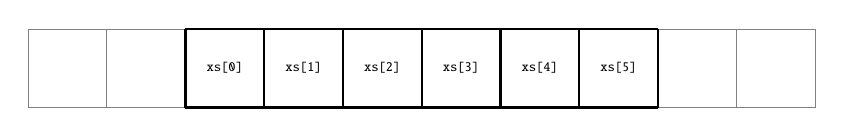
\begin{tikzpicture}
            \draw[help lines] (-2,0) grid (8,1);
            \draw[thick] (0,0) grid (6,1);
            \foreach \x in {0,...,5} {
                \node[font=\tiny] at ($ (\x,0.5) + (0.5,0) $) { \texttt{xs[\x]} };
            }
        \end{tikzpicture}
    \end{center}
    \vskip4mm
    \begin{itemize}
        \item One piece of contiguous memory
    \end{itemize}
\end{frame}

\begin{frame}
    \frametitle{Arrays}
    \code[language=c++14]{array.cpp}
\end{frame}

\begin{frame}
    \frametitle{Linked Lists}
    \begin{center}
        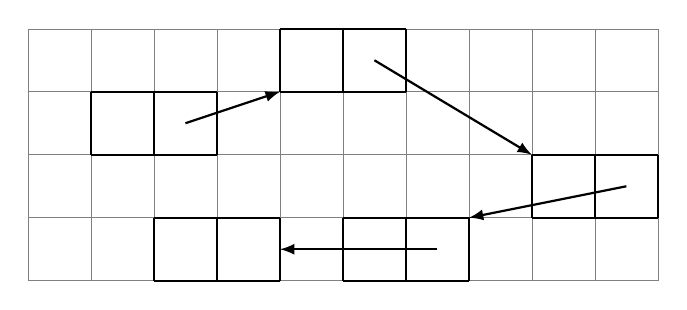
\begin{tikzpicture}[link/.style={thick,-latex},scale=0.8,transform shape]
            \draw[help lines] (0,0) grid (10,4);
            \draw[thick] (1,2) grid ++(2,1);
            \draw[thick] (4,3) grid ++(2,1);
            \draw[thick] (5,0) grid ++(2,1);
            \draw[thick] (2,0) grid ++(2,1);
            \draw[thick] (8,1) grid ++(2,1);

            \draw[link] (2.5,2.5) -- (4,3);
            \draw[link] (5.5,3.5) -- (8,2);
            \draw[link] (9.5,1.5) -- (7,1);
            \draw[link] (6.5,0.5) -- (4,0.5);
        \end{tikzpicture}
    \end{center}
    \vskip4mm
    \begin{itemize}
        \item List consists of series of nodes
        \item Each node has two fields
              \begin{itemize}
                \item Item
                \item Reference to next node
              \end{itemize}
        \item Nodes spread across memory
    \end{itemize}
\end{frame}

\begin{frame}
    \frametitle{Linked Lists in Code}
    \code[language=csharp]{LinkedList.cs}
\end{frame}

\begin{frame}
    \frametitle{Creating a Linked List}
    \begin{center}
        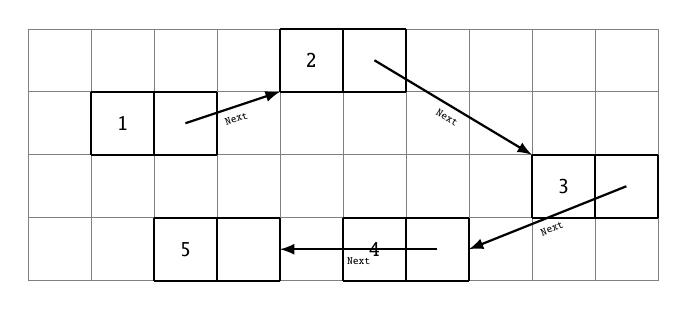
\begin{tikzpicture}[link/.style={thick,-latex},scale=0.8,transform shape]
            \draw[help lines] (0,0) grid (10,4);
            \draw[thick] (1,2) grid ++(2,1);
            \draw[thick] (4,3) grid ++(2,1);
            \draw[thick] (5,0) grid ++(2,1);
            \draw[thick] (2,0) grid ++(2,1);
            \draw[thick] (8,1) grid ++(2,1);

            \draw[link] (2.5,2.5) -- (4,3) node[midway,font=\tiny\ttfamily,sloped,below]{Next};
            \draw[link] (5.5,3.5) -- (8,2) node[midway,font=\tiny\ttfamily,sloped,below]{Next};
            \draw[link] (9.5,1.5) -- (7,0.5) node[midway,font=\tiny\ttfamily,sloped,below]{Next};
            \draw[link] (6.5,0.5) -- (4,0.5) node[midway,font=\tiny\ttfamily,sloped,below]{Next};

            \node[font=\ttfamily] at (1.5,2.5) {1};
            \node[font=\ttfamily] at (4.5,3.5) {2};
            \node[font=\ttfamily] at (8.5,1.5) {3};
            \node[font=\ttfamily] at (5.5,0.5) {4};
            \node[font=\ttfamily] at (2.5,0.5) {5};
        \end{tikzpicture}
    \end{center}
    \vskip4mm
    \code[language=csharp]{LinkedListCreation.cs}
\end{frame}

\section{Determining Length}

\frame{\tableofcontents[currentsubsection]}

\begin{frame}
    \frametitle{Length of Array}
    \begin{itemize}
        \item Array must keep track of Length
        \item Querying length is $O(1)$
    \end{itemize}
\end{frame}

\begin{frame}
    \frametitle{Length of Linked List}
    \begin{center}
        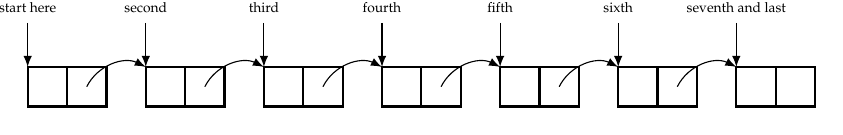
\begin{tikzpicture}[link/.style={thick,-latex}]
            \path[use as bounding box] (0,0) rectangle (10,1);

            \foreach[count=\i] \x in {0,1.5,...,10} {
                \coordinate (p\i) at (\x,0);
                \draw[thick] (p\i) rectangle ++(0.5,0.5);
                \draw[thick] ($ (p\i) + (0.5,0) $) rectangle ++(0.5,0.5);
            }

            \foreach[count=\i] \x in {0,1.5,...,8} {
                \draw[-latex] ($ (p\i) + (0.75,0.25) $) to[bend left=45] ++(0.75,0.251);
            }

            \foreach \i/\label in {1/{start here},2/{second},3/{third},4/{fourth},5/{fifth},6/{sixth},7/{seventh and last}} {
                \only<\i>{
                    \node[font=\tiny] (label) at ($ (p\i) + (0,1.25) $) {\label};
                    \draw[-latex] (label.south) -- ($ (p\i) + (0,.5) $);
                }
            }
        \end{tikzpicture}
    \end{center}
    \vskip4mm
    \structure{Algorithm}
    \begin{itemize}
        \item Follow nodes until we find \texttt{null}
        \item Count number of jumps necessary
        \item Takes longer for longer lists
    \end{itemize}
\end{frame}

\begin{frame}
    \frametitle{Indexing}
    \begin{center}
        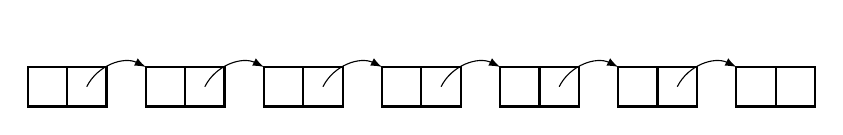
\begin{tikzpicture}[link/.style={thick,-latex}]
            \path[use as bounding box] (0,0) rectangle (10,1);

            \foreach[count=\i] \x in {0,1.5,...,10} {
                \coordinate (p\i) at (\x,0);
                \draw[thick] (p\i) rectangle ++(0.5,0.5);
                \draw[thick] ($ (p\i) + (0.5,0) $) rectangle ++(0.5,0.5);
            }

            \foreach[count=\i] \x in {0,1.5,...,8} {
                \draw[-latex] ($ (p\i) + (0.75,0.25) $) to[bend left=45] ++(0.75,0.251);
            }
        \end{tikzpicture}
    \end{center}
    \vskip4mm
    \structure{Algorithm}
    \begin{itemize}
        \item Follow \texttt{Next} \texttt{n} times
        \item Finding \texttt{n}th element takes \texttt{n} jumps
    \end{itemize}
\end{frame}

\begin{frame}
    \frametitle{Add to Front}
    \begin{center}
        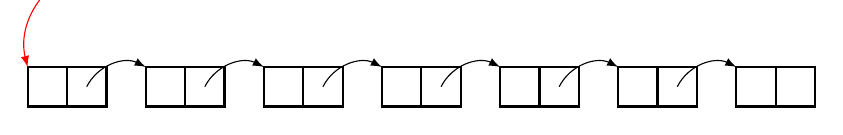
\begin{tikzpicture}[link/.style={thick,-latex}]
            \path[use as bounding box] (0,0) rectangle (10,1);

            \foreach[count=\i] \x in {0,1.5,...,10} {
                \coordinate (p\i) at (\x,0);
                \draw[thick] (p\i) rectangle ++(0.5,0.5);
                \draw[thick] ($ (p\i) + (0.5,0) $) rectangle ++(0.5,0.5);
            }

            \foreach[count=\i] \x in {0,1.5,...,8} {
                \draw[-latex] ($ (p\i) + (0.75,0.25) $) to[bend left=45] ++(0.75,0.251);
            }

            \only<2>{
                \coordinate (p0) at ($ (p1) + (0,1.5) $);
                \draw[red,thick] (p0) rectangle ++(0.5,0.5);
                \draw[red,thick] ($ (p0) + (0.5,0) $) rectangle ++(0.5,0.5);
                \draw[red,-latex] ($ (p0) + (0.75,0.25) $) to[bend right=45] ($ (p1) + (0,0.5) $);
            }
        \end{tikzpicture}
    \end{center}
    \vskip4mm
    \structure{Algorithm}
    \begin{itemize}
        \item Create new node
        \item Have it point to the (originally) first node
    \end{itemize}
\end{frame}

\begin{frame}
    \frametitle{Comparison}
    \begin{center}
        \begin{tabular}{lcc}
            & \textbf{Array} & \textbf{Linked List} \\
            \midrule
            Length & $O(1)$ & $O(n)$ \\
            Indexing & $O(1)$ & $O(n)$ \\
            Add to front & $O(n)$ & $O(1)$ \\
            Add to end & $O(n)$ & $O(n)$ \\
            Concatenation & $O(n_1+n_2)$ & $O(n_1)$ \\
            \bottomrule
        \end{tabular}
    \end{center}
\end{frame}

\end{document}

%%% Local Variables:
%%% mode: latex
%%% TeX-master: t
%%% End:
